\documentclass[12pt]{article}
\usepackage[utf8]{inputenc}
\usepackage[a4paper, margin=1in]{geometry}
\usepackage{titlesec}
%\usepackage[style=ieee, backend=biber]{biblatex}
\usepackage{graphicx}
\usepackage{amsmath}
\usepackage{amssymb}
\usepackage{amstext}
\usepackage{enumitem}
\usepackage{siunitx}
\usepackage{array}
\usepackage{xcolor}
\usepackage{multirow}
\usepackage{hyperref}
\usepackage{tabularx}
\usepackage{booktabs}
\usepackage{soul}
\usepackage{fancyhdr}
\usepackage{setspace}
%\usepackage{multicol}
\setlength{\columnsep}{.7cm}

\hypersetup{
    colorlinks=true,
    linkcolor=blue,
    filecolor=magenta,
    urlcolor=blue,
    pdftitle={aes670hw2},
    pdfpagemode=FullScreen,
    }
\urlstyle{same}

\newcolumntype{L}{>{$}l<{$}}  % Math mode table
\newcolumntype{R}{>{$}r<{$}}  % Math mode table
\newcolumntype{C}{>{$}c<{$}}  % Math mode table

\pagestyle{fancy}

\renewcommand{\sectionmark}[1]{%
\markboth{\thesection\quad #1}{}}
\fancyhead{}
\fancyhead[L]{\leftmark}
\fancyfoot{}
\fancyfoot[C]{\thepage}

\bibliographystyle{ieeetr}

\definecolor{Light}{gray}{.9}
\sethlcolor{Light}

\newcommand{\hltexttt}[1]{\texttt{\hl{#1}}}

\newcommand*{\problem}[2]{
    \begin{table}[ht]
    \centering
        \begin{tabular}{ | p{.1\linewidth} p{.9\linewidth} | }
            \hline
            \vspace{.3em}\textbf{\large#1:} & \vspace{.3em}\footnotesize{#2}\hspace{.2em}\vspace{.5em} \\ \hline
        \end{tabular}
    \end{table}
}

\newcommand\T{\rule{0pt}{2.6ex}}       % Top strut
\newcommand\B{\rule[-1.2ex]{0pt}{0pt}} % Bottom strut

\titleformat{\section}
  {\normalfont\fontsize{14}{15}\bfseries}{\thesection}{1em}{}

\titleformat{\subsection}
  {\normalfont\fontsize{12}{15}\bfseries}{\thesubsection}{1em}{}

\title{AES 770 Satellite Remote Sensing II

Smoke and Cloud Radiative Forcing}

\author{Mitchell Dodson}
\date{November 7, 2023}

\begin{document}

\maketitle

\vspace{-2em}

\begin{figure}[h!]
    \centering
    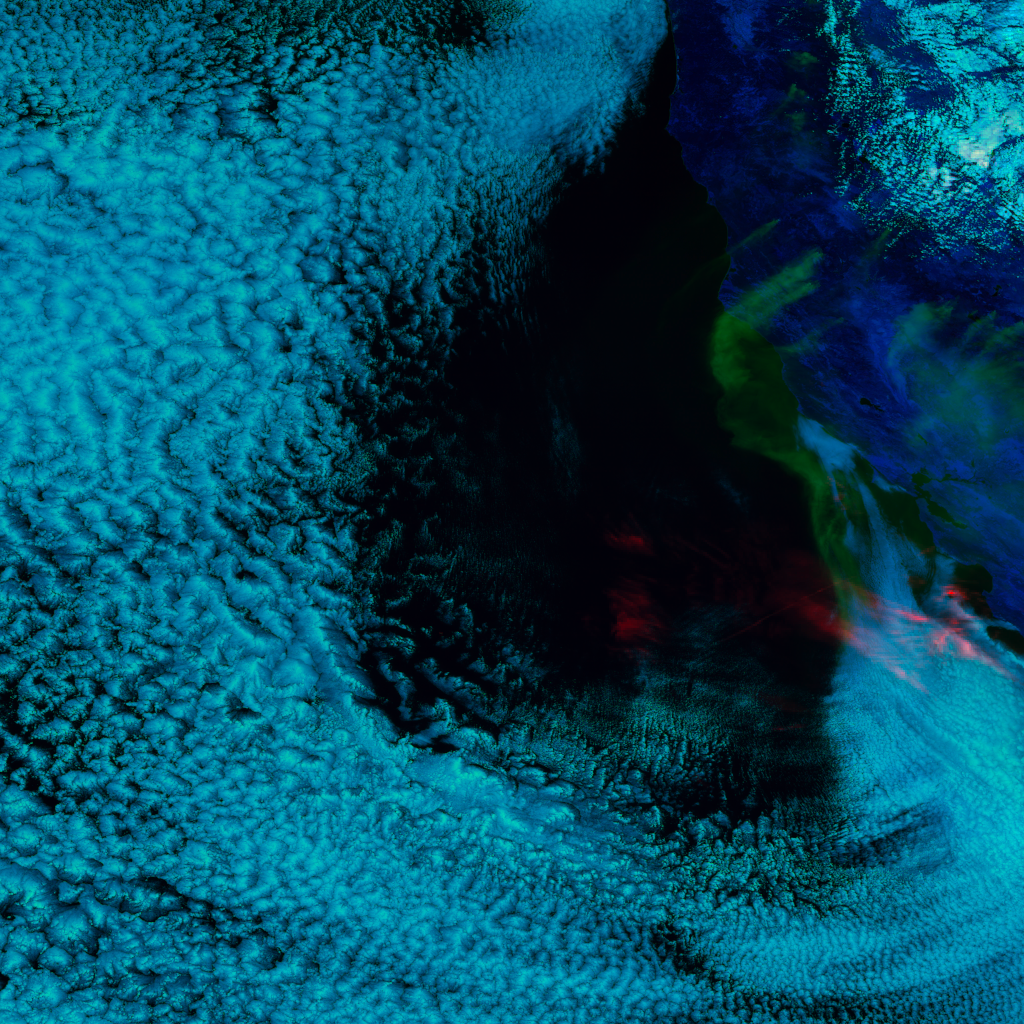
\includegraphics[width=.5\paperwidth]{figs/cover.png}
    \caption{GOES-17 ABI Daytime Cloud Phase RGB of the Region of Interest, captured on August 18, 2021 at 1910z. Light blue indicates warm water clouds, green indicates fine and uniform smoke particles, and red indicates cirrus cloud cover.}
    \label{cover}
\end{figure}

\vspace{-1em}

\section{Abstract}

In this report, I provide an assessment of the Cloud Radiative Forcing (CRF) and Aerosol Radiative Forcing (ARF) in both the longwave and shortwave spectral ranges using L2 Single-Scan Footprint (SSF) data from the Clouds and Earth Radiant Energy System (CERES) instrument, as well as co-located imager data from the Moderate Resolution Imaging Spectroradiometer (MODIS) instrument on the same satellite platforms, which are included with the SSF dataset. I focus on a Region of Interest (RoI) spanning $135^\circ W$ to $120^\circ W$ and $30^\circ N$ to $45^\circ N$, and the data I include consists of daytime overpasses from both the Terra and Aqua satellites between August 15 and August 25, 2021.


%\begin{multicols}{2}

\section{Introduction}

    Clouds and aerosols both play a significant role Earth's radiation budget, but remain two of the greatest sources of uncertainty in modeling climate sensitivity \cite{masson-delmotte_climate_2021}. Clouds are difficult to characterize for several reasons including that they typically have conflicting longwave and shortwave effects that depend on the type and the temperature of both a cloud and the surface it occludes. Additionally, the feedback mechanisms that affect changes in the global distribution of clouds with respect to changing temperatures remain unclear \cite{ramanathan_cloud-radiative_1989}. Aerosols also pose challenges to modeling because (1) their type and distribution is highly regionally and contextually variable, (2) they can facilitate cloud nucleation (the so-called indirect effect), and (3) because they can enhance the evaporation rate of a juxtaposed cloud layer due to warming by absorption (semi-direct effect)\cite{kaufman_satellite_2002}. What's more is that in both cases there are no reliable counterfactual observations for comparing results to a pre-industrial atmosphere, which makes the anthropogenic contribution to climate forcing difficult to quantify. As such, it's especially important to employ direct observational data of clear skies, aerosols, and full-sky outgoing fluxes with broadband instruments like the Earth Radiation Budget Experiment (ERBE) constellation, and more recently CERES.

    The setting for this study is a region covering the coast of central California over a 10-day period during a significant wildfire event. This is an appropriate choice for studying the radiative impact of clouds and smoke aerosols from biomass burning because the characteristic morning sea breeze consistently draws smoke aerosols out over the ocean, and facilitates the development of low-level stratocumulus clouds with a wide variety of optical depths. I restrict the data I use to only the daytime overpasses by Terra and Aqua, which are around 11:00am (19z) and 1:00pm (21z), respectively.

    For context, the 2021 California wildfire season was one of the worst on record, following a persistent drought that lasted throughout 2020 and until at least September of 2021. During this period of time, regional precipitation totals were the lowest since at least 1895 \cite{mankin_noaa_2021}, which culminated in 7,396 wildfires burning over 2,569,000 acres according to the California Wildfire Incident Archive \cite{the_department_of_forestry_and_fire_protection_2021_nodate}. Two of the most significant wildfire events were the Dixie and Caldor wildfires, which burned $963,309$ and $221,835$ acres respectively, mutually forced the evacuation of more than 29,000 residents, and were both the first known fires to cross the divide of the Sierra Nevada range \cite{chan_unprecedented_2021}\cite{the_department_of_forestry_and_fire_protection_2021_nodate}. The Caldor fire began conflagrating the High Sierra just West of Lake Tahoe on August 14 and rapidly grew over the following days, while the Dixie fire had already been burning further North since mid-July at the time of this study. These two forest fire events contributed much of the smoke considered in this study, and I personally witnessed the devastation and subsequent re-growth following the Caldor fire while backpacking the area in June 2023.

\begin{figure}[h!]\label{flux-interp}
    \centering
    \begin{center}
        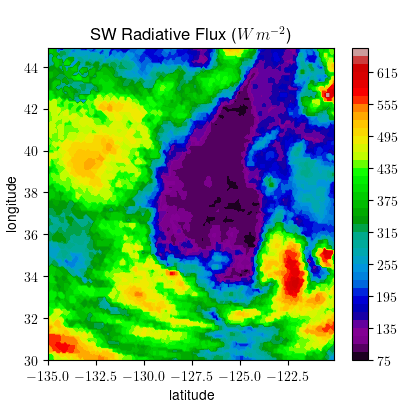
\includegraphics[width=.48\linewidth]{figs/interp_swflux.png}
        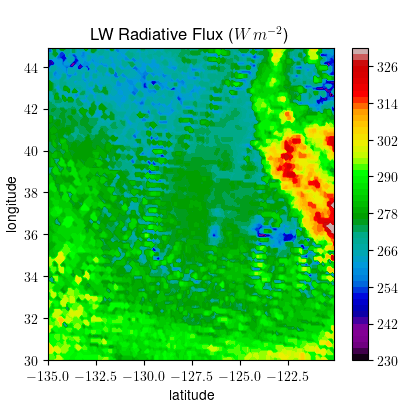
\includegraphics[width=.48\linewidth]{figs/interp_lwflux.png}
    \end{center}
    \caption{Outgoing Shortwave and Longwave fluxes observed by CERES on August 18, 2021 at 1910z (same swath as Figure \ref{cover}). The $\sim16\times32\,\si{km}$ footprints are resampled onto a uniform $0.1^\circ$ grid by nearest-neighbor interpolation.}
\end{figure}


\section{Background}

    \subsection{Cloud Radiative Forcing}

     Clouds have a substantial influence on the radiation budget due to their high reflectivity as well as emissivity. In the shortwave range, enhanced reflection of insolation causes a general cooling effect that is most prominent in the mid-latitude summer, and over bodies of water \cite{harrison_seasonal_1990}. This effect is clearly demonstrated by the broad-band shortwave flux in Figure \ref{flux-interp}, which shows that outgoing shortwave radiation over the highest-reflectivity water clouds exceeds that of the ocean surface by as much as $540\,\si{W.m^{-2}}$.

    The longwave impact of clouds is less prominent for liquid water clouds over the ocean since both surfaces have a comparable temperature and emissivity, however over land (in the top right of the second image in Figure \ref{flux-interp}), there is a stark depression in outgoing longwave radiation (OLR) associated with low-level water clouds. Furthermore, the thin cirrus clouds associated with red hues in the center-right of Figure \ref{cover} correspond to a decrease in OLR over the same area in Figure \ref{flux-interp}. Both of cases are indicative of the greenhouse effect of clouds which result in a net warming effect that is generally less prominent than the shortwave forcing.

    \subsection{Aerosol Radiative Forcing}

\begin{table}[h!]
    \centering
    \begin{tabular}{ m{.15\linewidth} | m{.15\linewidth} | m{0.6\linewidth}}
        \textbf{Parameter} & \textbf{Value} & \textbf{Justification} \\
        \hline
        & & \\
    \end{tabular}
    \caption{}
    \label{}
\end{table}

\section{Retrieval Methodology}

\subsection{Model Analysis}

\begin{figure}[h!]
    \centering
    \begin{center}
        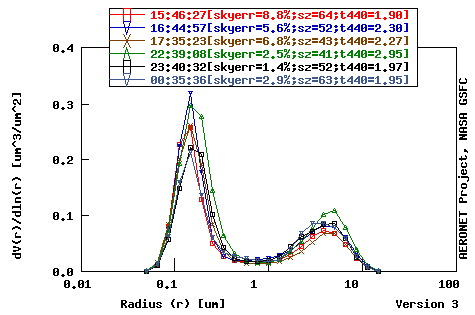
\includegraphics[width=.55\paperwidth]{figs/20210818_aeronet_ames_sdist.png}
        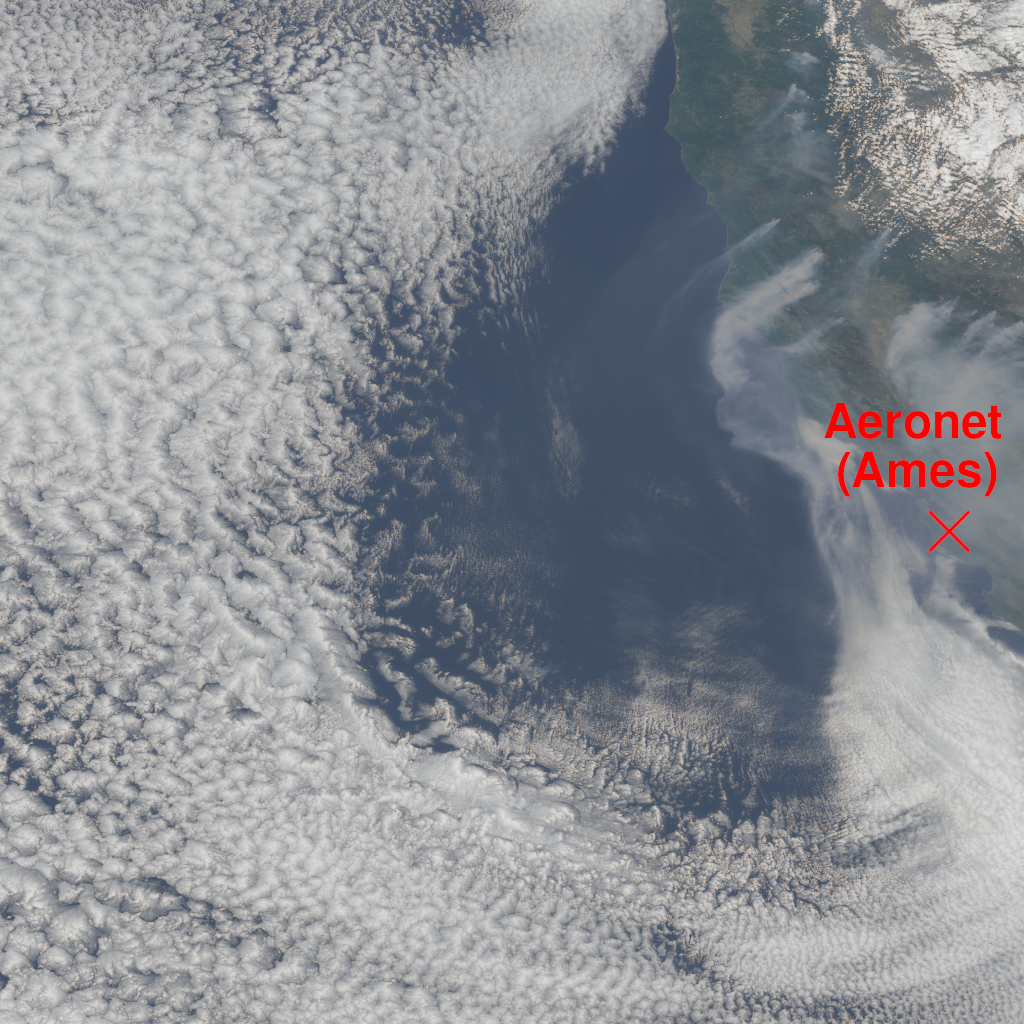
\includegraphics[width=.55\paperwidth]{figs/20210818_aeronet_marked-rgb.png}
    \end{center}
    \caption{}
    \label{}
\end{figure}

\subsection{Reference Pixel Selection}


\subsection{Aerosol Optical Depth Retrieval}

\section{Results}

\subsection{Validation Comment}

\subsection{Analysis}

\begin{table}[h!]\label{}
    \centering
    \begin{tabular}{ c c | c c c c c}
        & & & & & & \\
        \hline
        \multirow{4}*{} &
        & & & & & \T\\
        & & & & & \B\\
        \hline
        \multirow{2}*{Valid} &
        Meta & .2779 & .246 & .3684 & .4755 & .3923 \T\\
        &Grid & .2791 & .2495 & 2.270 & 2.378 & 2.292 \B\\
    \end{tabular}
    \caption{Comparison between my retrieval results and AOD values reported in the DESIS metadata, as well as the pixels in the AOD tiff grid corresponding to DDV values.}
\end{table}

%\end{multicols}

\section{Conclusion}

\bibliography{main}

\end{document}
